\documentclass[oneside,12pt]{article}
\usepackage{indentfirst}
\usepackage{fullpage}
\usepackage{blindtext, graphicx}
\usepackage{graphicx}
\usepackage[toc,page]{appendix}
\usepackage{lipsum}
\usepackage{booktabs}
\usepackage{caption}
\usepackage{tabularx}
\usepackage{amsmath}
\usepackage{gensymb}
\usepackage{tabu}
\usepackage{float}
\usepackage{url}
\usepackage{subfigure}
%\usepackage{listings}
\usepackage[framed,numbered]{matlab-prettifier}
\usepackage{color}
\usepackage[colorlinks=true,linkcolor=black, urlcolor=blue]{hyperref}
\setlength{\tabcolsep}{20pt}

\pagenumbering{gobble}



\begin{document}
\begin{titlepage}
	\begin{center}
		
		
\includegraphics[scale=0.7]{hulogo}\\
		\vspace{1cm}
		\large\textbf{ELE 613}\\
		\vspace{0.5cm}
		\large\textbf{SWITCH MODE POWER SUPPLIES}\\ 
		\vspace{0.5cm}
		
		\small\textbf{HOMEWORK 2}\\

		\vspace{0.5cm}
		
		\vspace{0.5cm}
		
		\line(1,0){400}\\
		\vspace{0.5cm}
	    \Large\textbf{HAKAN POLAT} 
	\end{center}
	

\end{titlepage}
\newpage
\section{Introduction}
This report shows the simulation results of a Forward Converter with the specs in Table \ref{my-label}.


\begin{table}[H]
	\centering
	\begin{tabular}{lll}
		Vin= 48V & Vo=5V      & n1/n2=4    \\
		n1/n3=1  & fs=100 kHz & Lm=200uH   \\
		Lr=40 uH & Cf=100uF   & Rl=0.5 ohm
	\end{tabular}
\caption{Forward Converters Specs}
\label{my-label}
\end{table}
The simulations are done in Matlab SIMULINK environment. The simulation model is in Fig \ref{fig:model}

\begin{figure}[H]
	\centering
	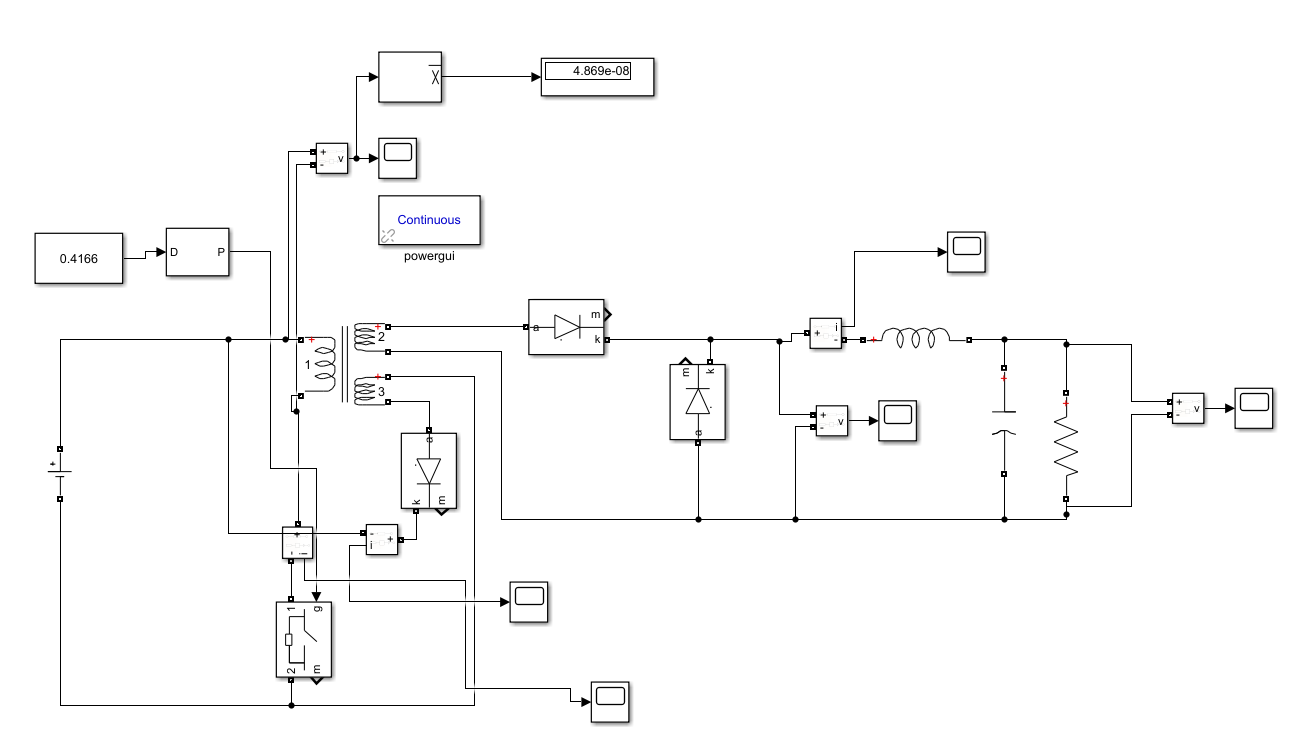
\includegraphics[width=0.8\linewidth]{model}
	\caption{Simulink model of forward converter}
	\label{fig:model}
\end{figure}

\section{Question 1}
According to the specs given the duty cycle $ D= 0.4166 $ for a 5V DC at the output. However this formula holds for the ideal, continious case which means no bias voltage of the diode. The simulations are done according to $ D= 0.4166 $ and hence the output voltage is 4.2 V with a 0.8V diode on voltage. The inductor current is in Figure \ref{fig:il} and the voltage input to the output stage (i.e voltage across D2) is in Figure \ref{fig:voi}

\begin{figure}[H]
	\centering
	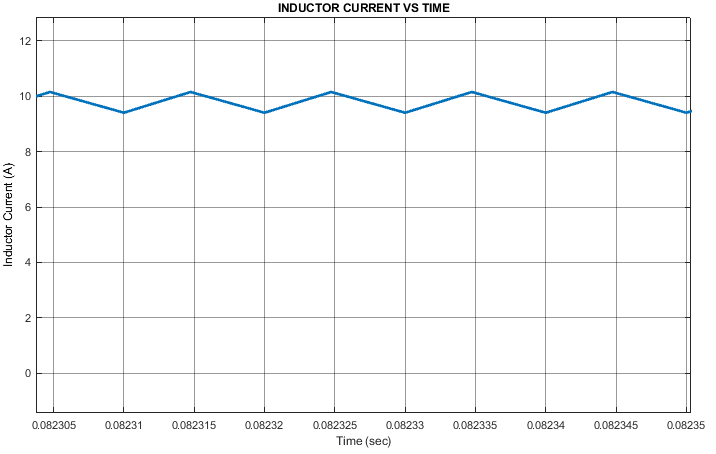
\includegraphics[scale=0.8]{../q1/i_L}
	\caption{Inductor Current}
	\label{fig:il}
\end{figure}


\begin{figure}[H]
	\centering
	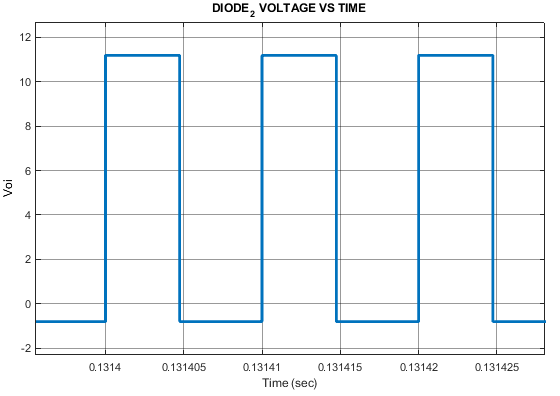
\includegraphics[scale=0.8]{../q1/Voi}
	\caption{$V_{oi}$ voltage}
	\label{fig:voi}
\end{figure}
\section{Question 2}
The V1 voltage is in Figure \ref{fig:v1}, the D3 current is in Figure \ref{fig:i3d3} and the switch current is in Figure \ref{fig:switch-current}.

\begin{figure}[H]
	\centering
	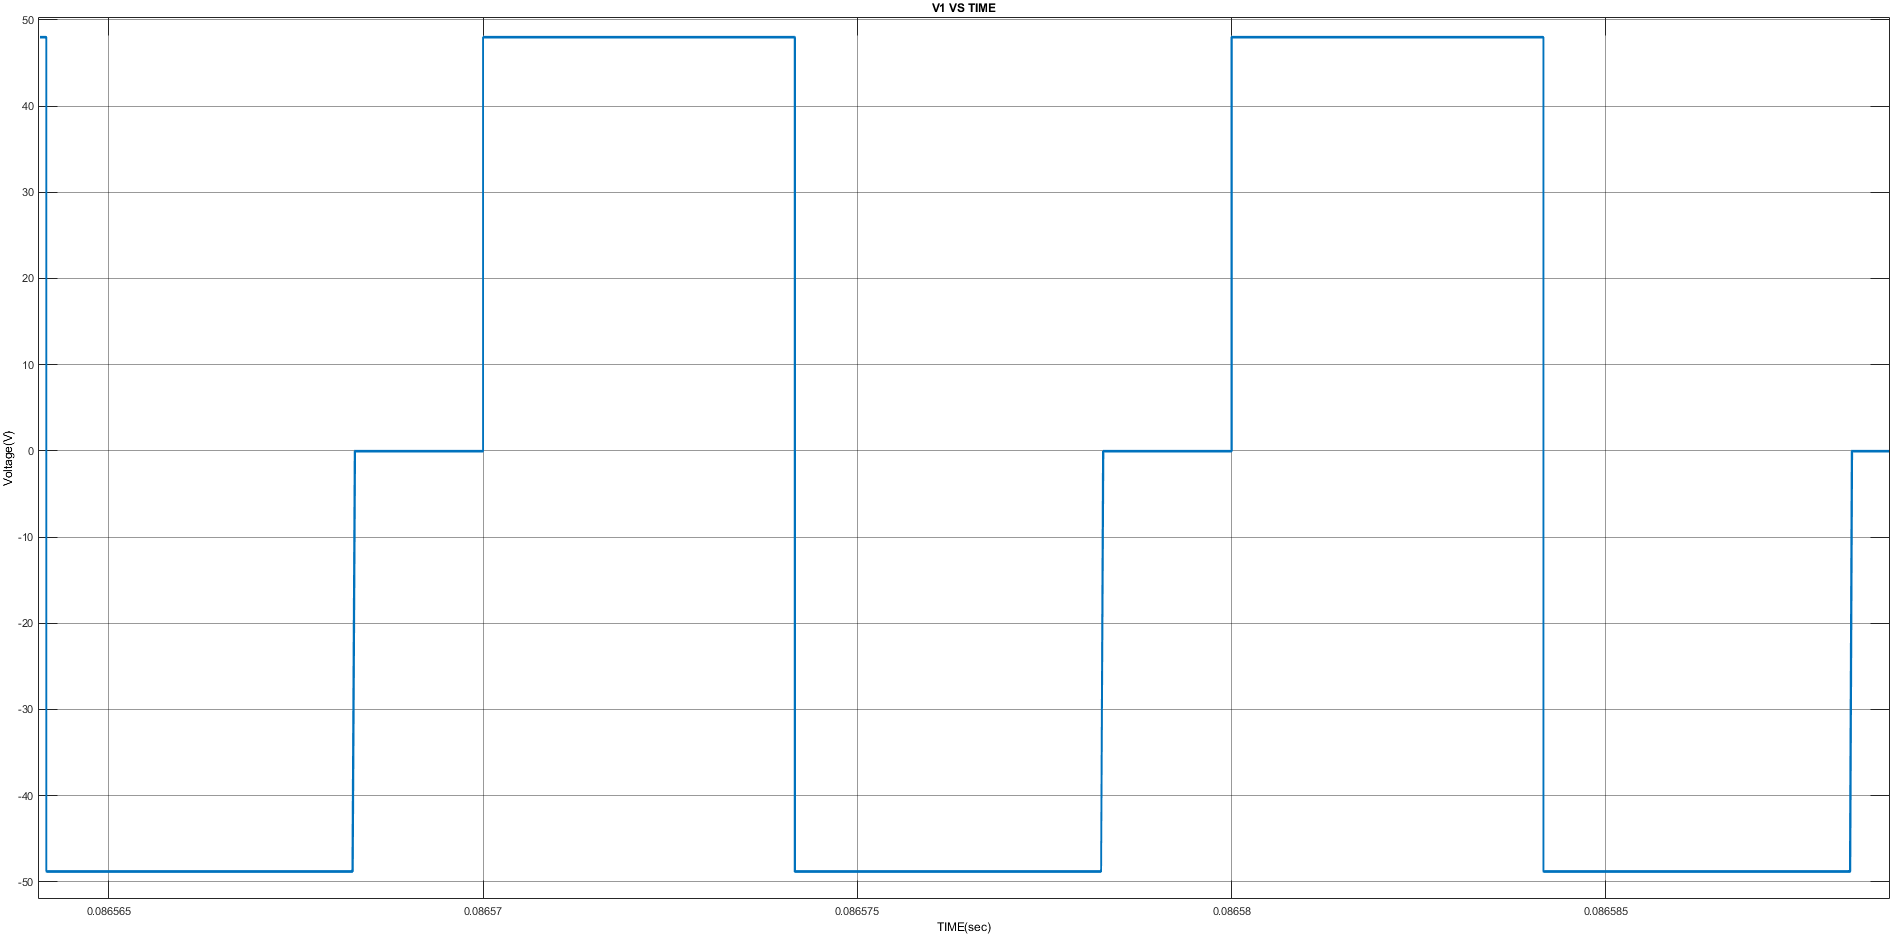
\includegraphics[scale=0.3]{../q2/v1}
	\caption{V1 voltage}
	\label{fig:v1}
\end{figure}

\begin{figure}[H]
	\centering
	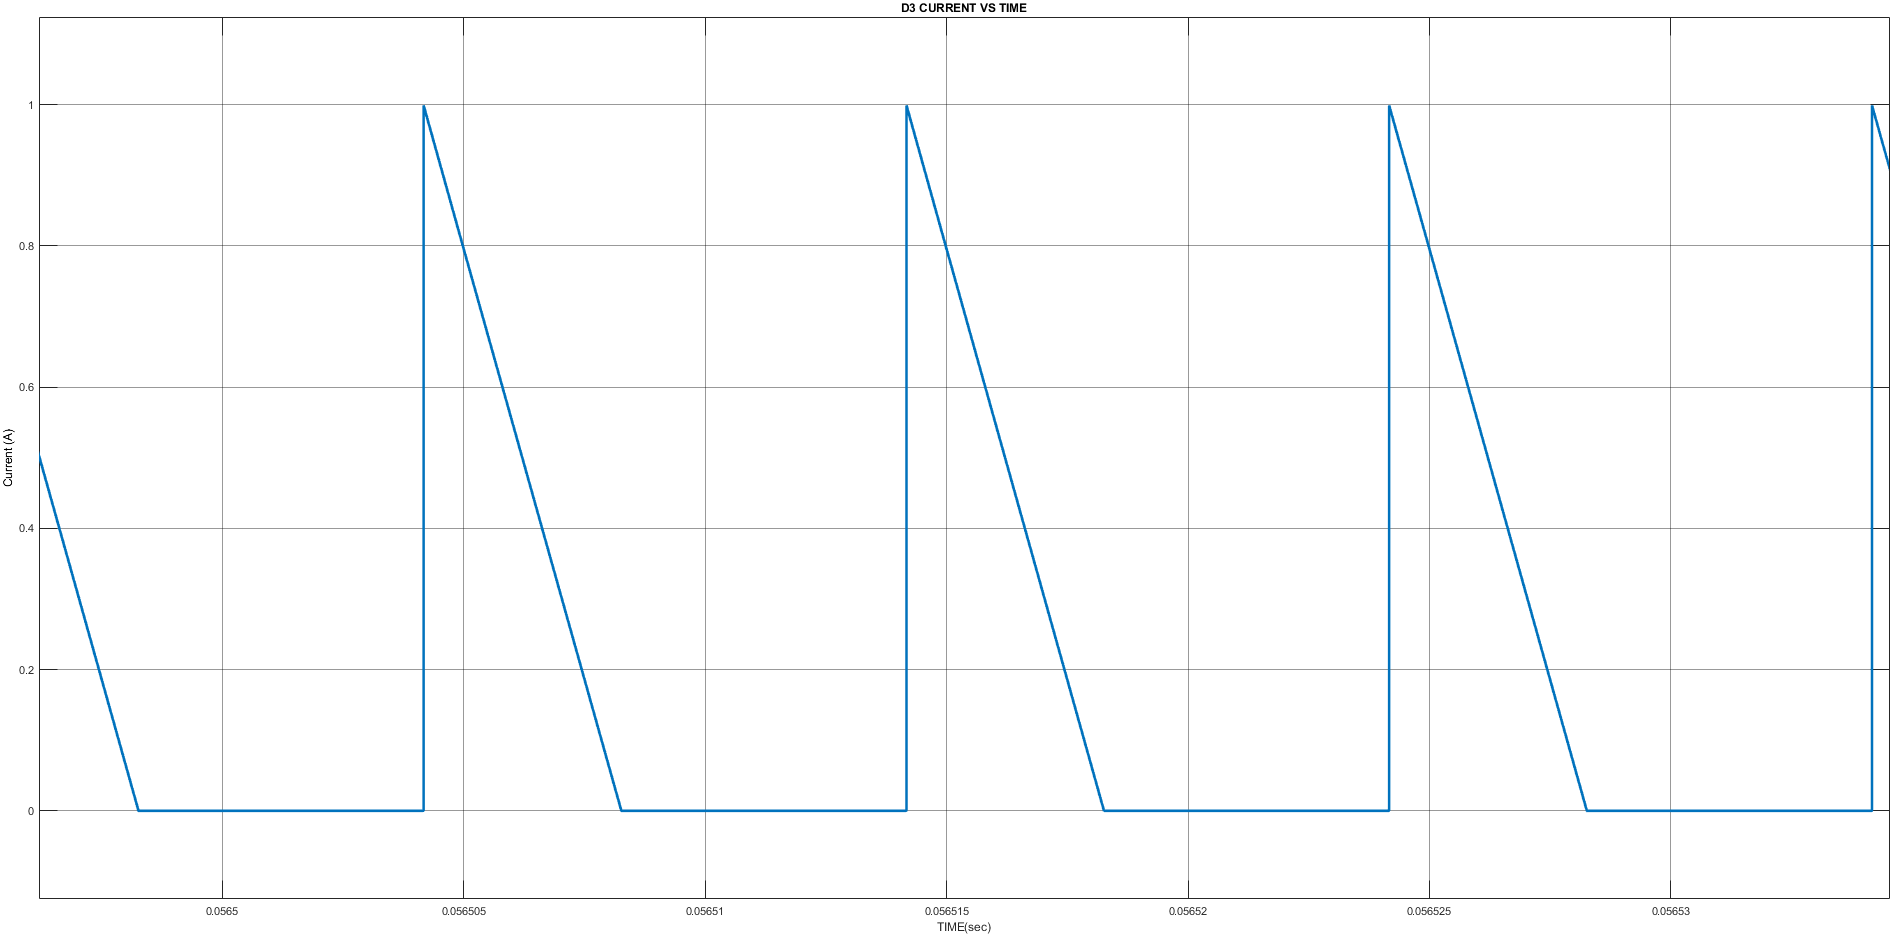
\includegraphics[scale=0.3]{../q2/i3_d3}
	\caption{D3 current}
	\label{fig:i3d3}
\end{figure}

\begin{figure}[H]
	\centering
	\includegraphics[scale=0.8]{"../q2/switch current"}
	\caption{Switch Current}
	\label{fig:switch-current}
\end{figure}


\section{Question 3}

\begin{figure}[H]
	\centering
	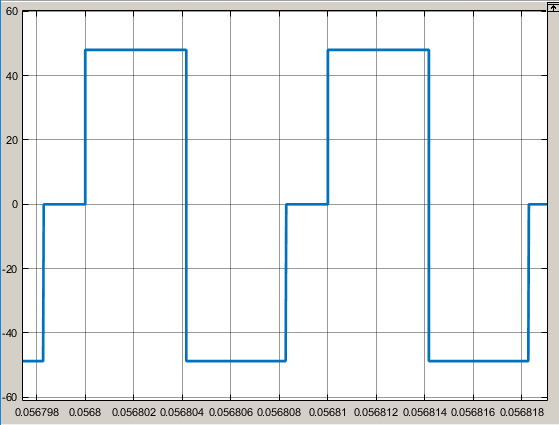
\includegraphics[width=0.7\linewidth]{../q3/v1_graph}
	\caption{V1 voltage}
	\label{fig:v1graph}
\end{figure}
 From Figure \ref{fig:v1graph}, we can observe that the magnitudes of positive and negative voltages are equal. Moreover we can measure the $ t_{1} $ and $ t_{2}$ corresponding to positive and negative voltage times. Hence;
 
 	\begin{equation}
 		V_{1,avg}= 0 V
 	\end{equation}
 	
 Using the simulation it is also possible to take the mean of any waveform. From Figure \ref{fig:v1avg} we can see that the V1 voltage is zero indeed expected from volt-seconds law of inductors.


\begin{figure}[H]
	\centering
	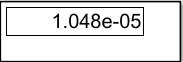
\includegraphics[scale=1]{../q3/v1_avg}
	\caption{Average of V1 measured in simulink}
	\label{fig:v1avg}
\end{figure}


\section{Question 4}
According to the formula since our $n1/n3=1$ the duty cycle and the times should hold. Our duty cycle $ D=0.4 $ meaning that tm should also be 0.4Ts. From  Figure \ref{fig:v1} it is clear that this formula is true.


\end{document}